\section{Results}
\label{sec:results}

Solve-rate and termination statistics come from \texttt{workspace/RESULTS/results.md}, produced by
\texttt{python3 workspace/aggregate\_results.py} over every saved run. 1,211% fact:results.attempts
attempts across 47 runs and 256 distinct samples. Every attempt is counted once, and an attempt with
no recorded \texttt{solved} field is counted as unsolved.

\paragraph{Crease-pattern distance.}
The saved-run CP-distance scan covers 1,422 attempts, of which 1,421 have recoverable
crease patterns. Mean insertion/deletion distance is 45.454; mean distance normalized
by target crease count is 0.553. One attempt is excluded because its state could not be
recovered. These averages pool models, baselines, configurations, and repeated samples;
they describe the saved attempts rather than a matched comparison of methods. This scan
includes runs outside the earlier 1,211-attempt solve-rate snapshot.
% EDITING NOTE: Refresh the paragraph above with summary.json when new runs are scored.
% Validate known complete, empty, partial, and wrong-assignment cases before submission.
\IfFileExists{../../workspace/RESULTS/cp-distance/paper-table.tex}{%
  \input{../../workspace/RESULTS/cp-distance/paper-table.tex}}{}

\subsection{Model performance}
\label{sec:results-headline}

\textbf{No language model solved a single sample beyond the easy group.} Across every model arm,
medium is 0 of 70 and hard is 0 of 27. On the easy group a deterministic breadth-first search over
exactly the action set the models are given solves 54.7\%, against 20.4\% for the best-covered model
at the same tier.

\begin{table}[h]
\caption{Solve rate per group, all saved runs. Denominators are attempts, not distinct samples.
Rows with fewer than ten attempts come from exploratory runs that were never extended into a
configured arm; they support no rate and are shown only so that reporting is not selective. The
single solved attempt by \texttt{gpt-6-astra} is one attempt, not a 100\% rate.}
\label{tab:headline}
\begin{center}
\footnotesize
\setlength{\tabcolsep}{2.5pt}
\begin{tabular}{llrrrrr}
\multicolumn{1}{c}{\bf ARM} &\multicolumn{1}{c}{\bf TIER} &\multicolumn{1}{c}{\bf EASY} &\multicolumn{1}{c}{\bf MEDIUM} &\multicolumn{1}{c}{\bf HARD} &\multicolumn{1}{c}{\bf OVERALL} &\multicolumn{1}{c}{\bf CALLS} \\
\hline \\
\texttt{deterministic-bfs} & legal-folds & {\bf 366/669 (54.7\%)} & 1/40 (2.5\%) & 0/16 & 367/725 (50.6\%) & 5 \\
\texttt{gpt-5.6-luna}      & legal-folds & 59/289 (20.4\%) & 0/66 & 0/25 & 59/380 (15.5\%) & 23.5 \\
\texttt{gpt-5.6-luna}      & basic tools & 4/65 (6.2\%)    & 0/1  & 0/1  & 4/67 (6.0\%)    & 29 \\
\texttt{claude-sonnet-5}   & legal-folds & 0/5  & -- & -- & 0/5 & 10 \\
\texttt{gpt-5.6-sol}       & basic tools & 0/7  & -- & -- & 0/7 & 20 \\
\texttt{gpt-5.6-terra}     & basic tools & 0/1  & -- & -- & 0/1 & 35 \\
\texttt{gpt-6-astra}       & basic tools & 1/1  & -- & -- & 1/1 & 5 \\
\texttt{codex-cli-chatgpt} & none        & 0/1  & -- & -- & 0/1 & 2 \\
\emph{errored, model unrecorded} & -- & 0/20 & 0/3 & 0/1 & 0/24 & -- \\
\end{tabular}
\end{center}
\end{table}

\textbf{Caveat: read the denominators before the percentages.} Only \texttt{gpt-5.6-luna} and the
baseline have coverage worth a rate. \texttt{gpt-6-astra} shows 1/1; \textbf{that is one attempt and
must not be reported as 100\%.} \texttt{claude-sonnet-5}, \texttt{gpt-5.6-sol},
\texttt{gpt-5.6-terra} and \texttt{codex-cli-chatgpt} have between one and seven attempts each.
These rows are present because omitting them would be selective reporting, not because they support
a comparison. Any main table in the submitted paper prints $n$ in every cell or drops the row.

\subsection{Search baseline}
\label{sec:results-baseline}

% Source: workspace/RESULTS/results.md, Deterministic search baseline.
% Static TeX bars; no additional plotting package or runtime required.
\begin{figure}[t]
\centering
\small
\begin{tabular}{llr}
Stratum (reference folds) & Median states expanded & Solved / attempts \\
\hline
Easy (4--10) & \rule{0.247cm}{8pt}\quad 65 & 366/669 \\
Medium (11--13) & \rule{4cm}{8pt}\quad 1,051.5 & 1/40 \\
Hard (14--19) & \rule{2.024cm}{8pt}\quad 532 & 0/16 \\
\end{tabular}
\caption{Observed BFS search effort in the saved aggregate. Bar lengths use a linear scale and
show median states expanded across attempts, including unsuccessful attempts. Budgets and repeated
samples are not standardized by this aggregate; 358 of 725 attempts terminated in timeout.
The lower hard-stratum median does not imply that hard instances require less search.
Reference depth is not minimum solution length.}
\label{fig:bfs-effort}
\end{figure}


\texttt{deterministic-bfs} solves 367 of 725 attempts overall. Per group: 366/669 easy, 1/40 medium,
0/16 hard. Median states expanded is 65 on easy, 1051.5 on medium, 532 on hard. 358% fact:results.bfs.timeouts
of its 725 attempts ended in timeout rather than exhaustion, so \textbf{50.6\% is a lower bound
under the baseline's time budget, not the ceiling of exhaustive search.} Timeouts also explain why
the hard median falls below the medium one: an attempt stopped by the clock contributes the states
it had expanded when it stopped, so the groups where the budget binds hardest report the smaller
counts. The medians describe observed effort under that budget and are not estimates of the search
each group requires.

Candidate enumeration filters for legality and compatibility with the target crease pattern, which
is a prune of roughly 570 times and leaves a branching factor near 3.5
(Section~\ref{sec:exp-baselines}). The baseline measures systematic exploration under that
filtering; its success rate does not by itself identify which reasoning abilities a model uses.

\phantomsection
\label{sec:results-tiers}

On easy instances, Luna solves 59/289 attempts (20.4\%) with candidate filtering and 4/65
(6.2\%) with basic tools. These are descriptive rates from unmatched attempt sets; controlled
comparisons and the remaining assistance experiments are pending.
% EDITING NOTE: Update this comparison after the remaining experiments.

\subsection{Failure analysis}
\label{sec:results-failures}

\begin{table}[h]
\caption{Termination reasons for \texttt{gpt-5.6-luna}, 447 attempts.}
\label{tab:terminations}
\begin{center}
\begin{tabular}{lrr}
\multicolumn{1}{c}{\bf TERMINATION} &\multicolumn{1}{c}{\bf $n$} &\multicolumn{1}{c}{\bf SHARE} \\
\hline \\
\texttt{state\_cycling}       & 215 & 48.1\% \\
\texttt{finished}             & 167 & 37.4\% \\
\texttt{turn\_budget}         & 47  & 10.5\% \\
\texttt{repetition\_detected} & 18  & 4.0\% \\
\end{tabular}
\end{center}
\end{table}

State cycling terminates 215 of 447 Luna attempts (48.1\%), while another 18 terminate with a
repetition label and 47 reach the turn budget. These labels describe stopping behavior rather
than proving the absence of reasoning. Repeated exploration without reaching the target indicates
ineffective search in those attempts; attributing it to state tracking or action selection
requires trajectory analysis. A \texttt{finished} label denotes submission, not necessarily success.

The harness defaults include a limit of three repetitions of the same action from the same
position and fifteen arrivals at the same position by any route. The latter is a revisit limit,
not a limit of fifteen distinct branches. Such limits can stop repeated exploration and must be
reported from each run's configuration rather than inferred from defaults. The aggregate table
does not separately identify all revisit-limit events.
% EDITING NOTE: Audit per-run cycle and revisit limits and classify capped exploration separately.

\phantomsection
\label{sec:results-difficulty}

No model attempt solves a medium or hard instance in the reported aggregate; BFS solves one
medium instance. This observation is consistent with greater search difficulty at larger reference
depths, but does not establish a causal effect of depth.

Coupling separates instances at equal depth, for the search baseline.
Table~\ref{tab:coupling} holds the fold count fixed and splits samples at a coupling of four.
Counts are samples rather than attempts: the baseline is deterministic and its attempts repeat
samples under different budgets, so an attempt-weighted rate would weight a sample by how often
it was re-run. Depths below eight are omitted because the baseline closes them at any coupling.
The separation it shows is consistent with the cost model of Section~\ref{sec:exp-baselines},
where a fold that cuts more layers raises both the branching factor and the cost of expanding
one node.

\begin{table}[h]
\caption{Samples solved, split by coupling at equal fold depth. Counts are distinct samples, not
attempts. Cells hold between six and twenty samples, which is too few for a rate to be read
closely; they are given as counts for that reason.}
\label{tab:coupling}
\begin{center}
\small
\begin{tabular}{lcccc}
& \multicolumn{2}{c}{\texttt{deterministic-bfs}} & \multicolumn{2}{c}{\texttt{gpt-5.6-luna}} \\
Fold depth & coupling $<4$ & coupling $\geq 4$ & coupling $<4$ & coupling $\geq 4$ \\
\hline \\
8  & 13/13 & 11/16 & 2/11 & 0/9 \\
9  & 8/10  & 5/20  & 0/7  & 0/10 \\
10 & 4/6   & 2/15  & 0/4  & 1/11 \\
\end{tabular}
\end{center}
\end{table}

\textbf{The model arm shows no comparable separation.} Its direction changes between depths and
every cell is single digits, so these data do not establish that coupling affects the model. The
failure analysis above points elsewhere, to revisiting states rather than to the difficulty of
any one fold. Samples were not assigned to coupling bins, so both readings are observational.

\phantomsection
\label{sec:results-threats}
The aggregate contains 725 BFS attempts and 447 Luna attempts, with much smaller counts for other
models. Recorded reasoning settings are low for 461 model attempts and absent for 25. Twenty-four
attempts with missing model identity ended in error and are reported separately as unsolved.
Per-sample repeat statistics and matched-budget comparisons remain to be reported.

% Included by sections/09-results.tex. Regenerate with
%   node workspace/figures/make_main_result_figure.mjs
% then copy workspace/figures/out/main_result.tex here and drop the standalone wrapper.
\begin{figure}[t]
\centering
\definecolor{vizA}{HTML}{2A78D6}
\definecolor{vizB}{HTML}{EB6834}
\definecolor{vizC}{HTML}{1BAF7A}
% Main result: solve rate per difficulty group.
% Generated by workspace/figures/make_main_result_figure.mjs
% Source: /Users/luxian/FoldOriganmi/workspace/RESULTS/results.md ("By model and tool tier")
% claude-sonnet-5 / tools=legal-folds: easy 0/5, medium --, hard --
% codex-cli-chatgpt / tools=none: easy 0/1, medium --, hard --
% deterministic-bfs / tools=legal-folds: easy 366/669, medium 1/40, hard 0/16
% gpt-5.6-luna / tools=legal-folds: easy 59/289, medium 0/66, hard 0/25
% gpt-5.6-luna / tools=none: easy 4/65, medium 0/1, hard 0/1
% gpt-5.6-sol / tools=none: easy 0/7, medium --, hard --
% gpt-5.6-terra / tools=none: easy 0/1, medium --, hard --
% gpt-6-astra / tools=none: easy 1/1, medium --, hard --
%
% Standalone: pdflatex main_result.tex
% In a paper: keep the tikzpicture, drop the documentclass wrapper.
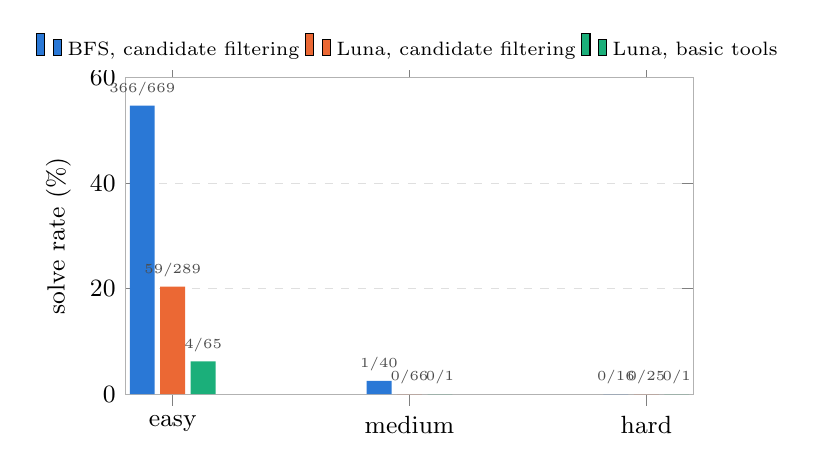
\begin{tikzpicture}
\begin{axis}[
  width=8.8cm, height=5.6cm,
  ybar, bar width=9pt,
  ymin=0, ymax=60,
  ylabel={solve rate (\%)},
  symbolic x coords={easy,medium,hard},
  xtick=data,
  point meta=explicit symbolic,
  nodes near coords={\pgfplotspointmeta},
  every node near coord/.append style={font=\tiny, color=black!70},
  tick label style={font=\small},
  label style={font=\small},
  legend style={font=\scriptsize, at={(0.5,1.16)}, anchor=north, legend columns=-1, draw=none},
  ymajorgrids, grid style={gray!25, dashed},
  axis line style={gray!60},
]
\addplot[fill=vizA, draw=none] coordinates {(easy,54.7) [366/669] (medium,2.5) [1/40] (hard,0.0) [0/16]};
\addlegendentry{BFS, candidate filtering}
\addplot[fill=vizB, draw=none] coordinates {(easy,20.4) [59/289] (medium,0.0) [0/66] (hard,0.0) [0/25]};
\addlegendentry{Luna, candidate filtering}
\addplot[fill=vizC, draw=none] coordinates {(easy,6.2) [4/65] (medium,0.0) [0/1] (hard,0.0) [0/1]};
\addlegendentry{Luna, basic tools}
\end{axis}
\end{tikzpicture}
\caption{\textbf{Solve rate by difficulty group.} Bars carry solved over attempts, and the
denominators are attempts rather than distinct samples, so one sample may be counted more
than once. The three arms shown are the ones with coverage enough to support a rate; the
five arms with fewer than ten attempts are omitted from the figure and account for 15
attempts, of which one was solved. Rates come from different sets of attempts and are not a
paired comparison on a matched sample set (Section~\ref{sec:results-threats}).}
\label{fig:main}
\end{figure}

